\documentclass[aspectratio=169,9pt]{beamer}
\mode<presentation> 
\usepackage[utf8]{inputenc}
\usepackage{sansmathaccent} %Für equations
\usepackage{amsmath}
\usepackage{tikz}
\usepackage{multicol}
\usepackage{cancel}
\usepackage{relsize}
\usepackage[table]{xcolor}
\usepackage[labelfont={bf},font={color=black!40,footnotesize},tablename={Tabelle},figurename={Abbildung}]{caption}
\usetikzlibrary{positioning, arrows.meta, calc}
\usefonttheme[onlymath]{serif}
%\makeatletter
%\makeatother

\rowcolors{2}{miugray!30}{miugray!10}

\usetheme{Madrid}  %% Themenwahl
\useoutertheme{split} % Alternatively: miniframes, infolines, split
%\useinnertheme{circles}


\setbeamertemplate{itemize item}{\color{miugray}$\blacksquare$}




\newcommand{\metermilli}{\mskip3mu \text{mm}}
\newcommand{\cm}{\mskip3mu \text{cm}}
\newcommand{\m}{ \text{m}}
\newcommand{\lite}{ \text{l}}
\newcommand{\kg}{ \text{kg}}
\newcommand{\g}{ \text{g}}
\newcommand{\km}{ \text{km}}
\newcommand{\h}{ \text{h}}
\newcommand{\s}{ \text{s}}
\newcommand{\tonne}{ \text{t}}

\newcommand{\RA}{$\rightarrow$~}
\newcommand{\pp}{\par \vspace*{2mm}}
\newcommand{\ppbig}{\par \vspace*{4mm}}

\definecolor{miudiutex}{HTML}{1d2926}
\definecolor{miugray}{HTML}{b4cccf}
\definecolor{miugray2}{HTML}{4d7365}
\definecolor{white2}{HTML}{f5f7f8}
\definecolor{red}{HTML}{cf1f5c}
\definecolor{green}{HTML}{00A36C}
\definecolor{delphinidin}{HTML}{315794}
\definecolor{uniblau}{HTML}{004e9f}
\definecolor{unigelb}{HTML}{fcba00}
\definecolor{unigrau}{HTML}{909085}
\definecolor{pelargonidin}{HTML}{b33807}
\definecolor{cyanidin}{HTML}{ba0746}
\definecolor{paeonidin}{HTML}{d15ca6}
\definecolor{petunidin}{HTML}{b56fed}
\definecolor{malvidin}{HTML}{8a2d8c}

%\setbeamercolor{palette primary}{bg=pelargonidin!35,fg=white}
%\setbeamercolor{palette secondary}{bg=delphinidin!45,fg=white}
\setbeamercolor{palette primary}{bg=uniblau!70,fg=white}
\setbeamercolor{palette secondary}{bg=uniblau!45,fg=white}
\setbeamercolor{palette tertiary}{bg=unigelb!70,fg=unigrau}
\setbeamercolor{palette quaternary}{bg=miugray,fg=white}
\setbeamercolor{structure}{fg=black} % itemize, enumerate, etc
\setbeamercolor{section in toc}{fg=uniblau} % TOC sections
\setbeamercolor{alerted text}{fg=uniblau}
\setbeamerfont{alerted text}{series=\bfseries}
\setbeamersize{text margin left=2cm,text margin right=2cm}


\useinnertheme{tcolorbox} 
\newcommand{\goodtk}[2]{
\begin{tcolorbox}[
	enhanced,
	colframe=uniblau!75,
	sharp corners,
	boxsep=5pt,
	title=\bfseries \sffamily #1,
	colback=white,
	coltitle=black,
	attach boxed title to top text left={yshift=-\tcboxedtitleheight/2},
	boxed title style={colback=white,colframe=white}
]
	#2
	\end{tcolorbox}
}
	
\newcommand{\goodtl}[2]{
\begin{tcolorbox}[
	enhanced,
	colframe=unigrau!65,
	sharp corners,
	boxsep=5pt,
	title=\bfseries \sffamily #1,
	colback=white,
	coltitle=black,
	attach boxed title to top text left={yshift=-\tcboxedtitleheight/2},
	boxed title style={colback=white,colframe=white}
]
	#2
	\end{tcolorbox}
}
\newcommand{\antwort}[1]{
\begin{tcolorbox}[
	enhanced,
	colframe=unigrau!65,
	sharp corners,
	boxsep=1pt,
	colback=white,
	coltitle=black,
]
	#1
	\end{tcolorbox}
}



\title{1. Übung pLMT}
\author{Sam Knorr}
\date{\today}

\begin{document}
%\maketitle

%\section{Einführung}
\begin{frame}

\begin{center}
Thema: \par 
\Huge 
Allgemeine Grundlagen 
\pp
\normalsize
Dichte, Konzentrationen \& Massenbilanzen
\end{center}

\end{frame}


\section{Dichte}


\begin{frame}
\footnotesize

\textbf{Aufgabe 1 a)} \pp
\begin{multicols}{2}
\begin{itemize}
\item Wie ist die Dichte eines Körpers definiert? \par  \pause
\antwort{Die Dichte eines Stoffes ist der Quotient aus der Masse $m$ des Körpers und seinem Volumen $V$.
\begin{align*}
\frac{m}{V}
\end{align*}
} 
\pause
\item Welches Formelzeichen wird für die Dichte verwendet? \par \pause
\antwort{$\rho$} \pause
\item Welche SI-Einheit hat sie? \par \pause
\antwort{kg/m$^3$} \pause
\item Ist die Dichte eine extensive oder intensive Größe? \par \pause
\antwort{Es handelt sich um eine \textbf{intensive} Größe, da sie unabhängig
von Form und Größe des Körpers ist.}

\end{itemize}

\end{multicols}
\end{frame}

%\begin{frame}
%
%\textbf{Aufgabe 1 b)}
%\pp
%\resizebox{.9\textwidth}{!}{
%\begin{tikzpicture}[font=\sffamily]
%
%  % --- Gemeinsame Stile definieren ---
%  \tikzset{
%    % Stil für die Kopfzeilen-Zellen
%    headercell/.style={rectangle, fill=miugray, text=black, font=\bfseries, minimum height=2.2em, align=center, inner sep=6pt},
%    % Stil für die linken Datenzeilen-Zellen (Text)
%    bodycell/.style={rectangle, fill=miugray!50, draw=white, minimum height=2.2em, align=left, inner sep=6pt},
%    % Stil für die rechten Datenzeilen-Zellen (Zahlen)
%    rightbodycell/.style={rectangle, fill=miugray!50, draw=white, minimum height=2.2em, align=center, inner sep=6pt},
%    % Stil für die kreisförmigen Verbindungsknoten
%    connectnode/.style={circle, draw=miugray, fill=white, inner sep=0pt, minimum size=7pt, anchor=center}
%  }
%
%  % ==========================================
%  %   LINKE SPALTE (Lebensmittelbestandteil)
%  % ==========================================
%  \node (head_left) [headercell, minimum width=6cm] {Lebensmittelbestandteil};
%
%  % Datenzeile: Fett
%  \node (fett) [bodycell, minimum width=6cm, below=-\pgflinewidth of head_left] {Fett};
%  \node (fett_conn) [connectnode] at (fett.east) {};
%
%  % Datenzeile: Protein
%  \node (protein) [bodycell, minimum width=6cm, below=-\pgflinewidth of fett] {Protein};
%  \node (protein_conn) [connectnode] at (protein.east) {};
%
%  % Datenzeile: Stärke
%  \node (staerke) [bodycell, minimum width=6cm, below=-\pgflinewidth of protein] {Stärke};
%  \node (staerke_conn) [connectnode] at (staerke.east) {};
%
%  % Datenzeile: Salz
%  \node (salz) [bodycell, minimum width=6cm, below=-\pgflinewidth of staerke] {Salz};
%  \node (salz_conn) [connectnode] at (salz.east) {};
%
%  % Datenzeile: Wasser
%  \node (wasser) [bodycell, minimum width=6cm, below=-\pgflinewidth of salz] {Wasser};
%  \node (wasser_conn) [connectnode] at (wasser.east) {};
%
%
%  % ==========================================
%  %      RECHTE SPALTE (Dichte)
%  % ==========================================
%  % Horizontale Positionierung relativ zur linken Spalte
%  \node (head_right) [headercell, minimum width=4cm, right=2.0cm of head_left.east, anchor=west] {Dichte};
%
%  % Datenzeile: 900 - 950
%  \node (dichte1) [rightbodycell, minimum width=4cm, below=-\pgflinewidth of head_right] {900 - 950};
%  \node (dichte1_conn) [connectnode] at (dichte1.west) {};
%
%  % Datenzeile: 1000
%  \node (dichte2) [rightbodycell, minimum width=4cm, below=-\pgflinewidth of dichte1] {1.000};
%  \node (dichte2_conn) [connectnode] at (dichte2.west) {};
%
%  % Datenzeile: ca. 1400
%  \node (dichte3) [rightbodycell, minimum width=4cm, below=-\pgflinewidth of dichte2] {ca. 1.400};
%  \node (dichte3_conn) [connectnode] at (dichte3.west) {};
%
%  % Datenzeile: 1500
%  \node (dichte4) [rightbodycell, minimum width=4cm, below=-\pgflinewidth of dichte3] {1.500};
%  \node (dichte4_conn) [connectnode] at (dichte4.west) {};
%
%  % Datenzeile: 2160
%  \node (dichte5) [rightbodycell, minimum width=4cm, below=-\pgflinewidth of dichte4] {2.160};
%  \node (dichte5_conn) [connectnode] at (dichte5.west) {};
%
%  % ==========================================
%  %      VERBINDUNGSLINIEN ZEICHNEN
%  % ==========================================
%  % Zeichnet eine saubere Linie für das im Bild gezeigte Beispiel (Wasser -> Protein/1000)
%  \draw[ultra thick, uniblau] (wasser_conn) -- (dichte2_conn);
%
%
%  % Optional: Wenn du weitere Linien hinzufügen möchtest, nutze diese Syntax:
%  % \draw[thick, gray] (fett_conn) -- (dichte1_conn);
%
%\end{tikzpicture}
%}
%
%\end{frame}




\begin{frame}

\textbf{Aufgabe 1 b)}
\pp
\resizebox{.9\textwidth}{!}{
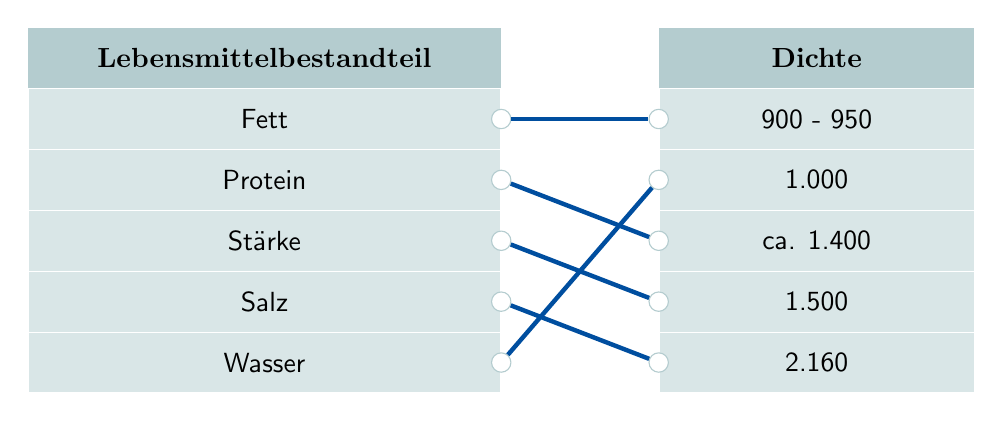
\begin{tikzpicture}[font=\sffamily]

  % --- Gemeinsame Stile definieren ---
  \tikzset{
    % Stil für die Kopfzeilen-Zellen
    headercell/.style={rectangle, fill=miugray, text=black, font=\bfseries, minimum height=2.2em, align=center, inner sep=6pt},
    % Stil für die linken Datenzeilen-Zellen (Text)
    bodycell/.style={rectangle, fill=miugray!50, draw=white, minimum height=2.2em, align=left, inner sep=6pt},
    % Stil für die rechten Datenzeilen-Zellen (Zahlen)
    rightbodycell/.style={rectangle, fill=miugray!50, draw=white, minimum height=2.2em, align=center, inner sep=6pt},
    % Stil für die kreisförmigen Verbindungsknoten
    connectnode/.style={circle, draw=miugray, fill=white, inner sep=0pt, minimum size=7pt, anchor=center}
  }

  % ==========================================
  %   LINKE SPALTE (Lebensmittelbestandteil)
  % ==========================================
  \node (head_left) [headercell, minimum width=6cm] {Lebensmittelbestandteil};

  % Datenzeile: Fett
  \node (fett) [bodycell, minimum width=6cm, below=-\pgflinewidth of head_left] {Fett};
  \node (fett_conn) [connectnode] at (fett.east) {};

  % Datenzeile: Protein
  \node (protein) [bodycell, minimum width=6cm, below=-\pgflinewidth of fett] {Protein};
  \node (protein_conn) [connectnode] at (protein.east) {};

  % Datenzeile: Stärke
  \node (staerke) [bodycell, minimum width=6cm, below=-\pgflinewidth of protein] {Stärke};
  \node (staerke_conn) [connectnode] at (staerke.east) {};

  % Datenzeile: Salz
  \node (salz) [bodycell, minimum width=6cm, below=-\pgflinewidth of staerke] {Salz};
  \node (salz_conn) [connectnode] at (salz.east) {};

  % Datenzeile: Wasser
  \node (wasser) [bodycell, minimum width=6cm, below=-\pgflinewidth of salz] {Wasser};
  \node (wasser_conn) [connectnode] at (wasser.east) {};


  % ==========================================
  %      RECHTE SPALTE (Dichte)
  % ==========================================
  % Horizontale Positionierung relativ zur linken Spalte
  \node (head_right) [headercell, minimum width=4cm, right=2.0cm of head_left.east, anchor=west] {Dichte};

  % Datenzeile: 900 - 950
  \node (dichte1) [rightbodycell, minimum width=4cm, below=-\pgflinewidth of head_right] {900 - 950};
  \node (dichte1_conn) [connectnode] at (dichte1.west) {};

  % Datenzeile: 1000
  \node (dichte2) [rightbodycell, minimum width=4cm, below=-\pgflinewidth of dichte1] {1.000};
  \node (dichte2_conn) [connectnode] at (dichte2.west) {};

  % Datenzeile: ca. 1400
  \node (dichte3) [rightbodycell, minimum width=4cm, below=-\pgflinewidth of dichte2] {ca. 1.400};
  \node (dichte3_conn) [connectnode] at (dichte3.west) {};

  % Datenzeile: 1500
  \node (dichte4) [rightbodycell, minimum width=4cm, below=-\pgflinewidth of dichte3] {1.500};
  \node (dichte4_conn) [connectnode] at (dichte4.west) {};

  % Datenzeile: 2160
  \node (dichte5) [rightbodycell, minimum width=4cm, below=-\pgflinewidth of dichte4] {2.160};
  \node (dichte5_conn) [connectnode] at (dichte5.west) {};

  % ==========================================
  %      VERBINDUNGSLINIEN ZEICHNEN
  % ==========================================
  % Zeichnet eine saubere Linie für das im Bild gezeigte Beispiel (Wasser -> Protein/1000)
  \draw[ultra thick, uniblau] (wasser_conn) -- (dichte2_conn);
\onslide<2->{\draw[ultra thick, uniblau] (fett_conn) -- (dichte1_conn);}
\onslide<3->{	\draw[ultra thick, uniblau] (protein_conn) -- (dichte3_conn);}
\onslide<4->{	\draw[ultra thick, uniblau] (staerke_conn) -- (dichte4_conn);}
\onslide<5->{	\draw[ultra thick, uniblau] (salz_conn) -- (dichte5_conn);}

  % Optional: Wenn du weitere Linien hinzufügen möchtest, nutze diese Syntax:
  % \draw[thick, gray] (fett_conn) -- (dichte1_conn);

\end{tikzpicture}
}

\end{frame}

\begin{frame}
\textbf{Aufgabe 1 c)}
\pp
\small
\begin{minipage}{.5\textwidth}
Bei porösen Festkörpern wird zwischen der sogenannten Reindichte
und der Rohdichte unterschieden. Die Rohdichte ist die Dichte des
Festkörpers basierend auf dem Volumen einschließlich der Porenräume.
Die Reindichte bezieht sich auf die Dichte des stofflichen Teils des
Körpers, ohne etwaige Hohlräume zu berücksichtigen.
\pp 
Stellen Sie die Formeln zur Berechnung der Roh- und der Reindichte
auf
\end{minipage}%
\hspace*{4mm}
\begin{minipage}{.5\textwidth}\pause

\antwort{
\begin{align*}
&\text{Rohdichte:}~{\mathlarger \rho}_{roh} &&= \frac{m}{V_{Stoff} + V_{por}} \\
&\text{Reindichte:}~{\mathlarger \rho}_{rein} &&= \frac{m}{V_{Stoff}}
\end{align*}
\pp
\footnotesize
$m$ : Masse des Festkörpers \par 
$V_{Stoff}$ : Volumen des Stoffes \par 
$ V_{por}$ : Volumen der Poren
}
\end{minipage}

\end{frame}



%\begin{frame}
%\textbf{Aufgabe 1 c)}
%\pp
%\small
%\begin{minipage}{.5\textwidth}
%Rohdichte vs. Reindichte \pp
%
%Rohdichte: Dichte \textbf{mit} Porenvolumen \par 
%Reindichte: Dichte \textbf{ohne} Porenvolumen
%\pp 
%Stellen Sie die Formeln zur Berechnung der Roh- und der Reindichte
%auf
%\end{minipage}%
%\hspace*{4mm}
%\begin{minipage}{.5\textwidth}\pause
%
%\antwort{
%\begin{align*}
%{\mathlarger \rho}_{roh} &= \frac{m}{V_{Stoff} + V_{por}} \\
%{\mathlarger \rho}_{rein} &= \frac{m}{V_{Stoff}}
%\end{align*}
%\pp
%\footnotesize
%$m$ : Masse des Festkörpers \par 
%$V_{Stoff}$ : Volumen des Stoffes \par 
%$ V_{por}$ : Volumen der Poren
%}
%\end{minipage}
%
%\end{frame}
%





\begin{frame}
\textbf{Aufgabe 1 d)}
\pp
\small
\begin{minipage}{.5\textwidth}
Die Schüttdichte bezeichnet die Dichte eines Gemenges aus einem körnigen Feststoff und einem kontinuierlichen Fluid. Stellen Sie die Formel zur Berechnung der Schüttdichte auf.
\pp 
Stellen Sie die Formeln zur Berechnung der Schüttdichte auf
\end{minipage}%
\hspace*{4mm}
\begin{minipage}{.5\textwidth}\pause
\antwort{
\begin{align*}
{\mathlarger \rho}_{Sch} &= \frac{m}{V_{Sch}}
\end{align*}
}
\end{minipage}
\end{frame}

\begin{frame}[fragile]{Vergleich der Dichten}
\begin{center}
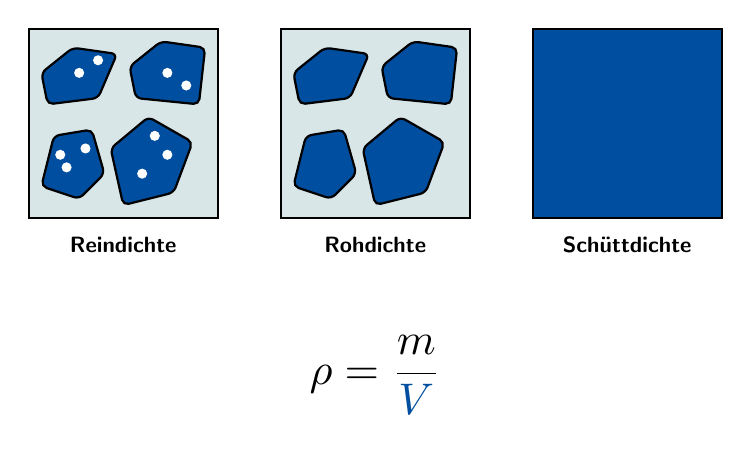
\begin{tikzpicture}[thick, font=\sffamily, scale=0.8, transform shape] 
    % scale=0.8 verkleinert die Grafik leicht, damit sie gut auf die Folie passt

    % --- 1. REINDICHTE ---
    \begin{scope}[shift={(0,0)}]
        \fill[miugray!50] (0,0) rectangle (3,3);
        % Partikel füllen und zuschneiden (hartcodierte Koordinaten)
        \begin{scope}
            \clip[rounded corners=2pt] 
                (0.2, 0.5) -- (0.8, 0.3) -- (1.2, 0.7) -- (1.0, 1.4) -- (0.4, 1.3) -- cycle
                (1.5, 0.2) -- (2.3, 0.4) -- (2.6, 1.2) -- (1.9, 1.6) -- (1.3, 1.1) -- cycle
                (0.3, 1.8) -- (1.1, 1.9) -- (1.4, 2.6) -- (0.7, 2.7) -- (0.2, 2.3) -- cycle
                (1.7, 1.9) -- (2.7, 1.8) -- (2.8, 2.7) -- (2.1, 2.8) -- (1.6, 2.4) -- cycle;
            
            \fill[uniblau] (0,0) rectangle (3,3);
            
            % Innere Poren (weiß aussparen)
            \foreach \p in {(0.6,0.8), (0.9,1.1), (0.5,1.0), (1.8,0.7), (2.2,1.0), (2.0,1.3), (0.8,2.3), (1.1,2.5), (2.2,2.3), (2.5,2.1)}
                \fill[white] \p circle (0.08);
        \end{scope}
        
        % Umrisse zeichnen (hartcodierte Koordinaten)
        \draw[rounded corners=2pt] 
                (0.2, 0.5) -- (0.8, 0.3) -- (1.2, 0.7) -- (1.0, 1.4) -- (0.4, 1.3) -- cycle
                (1.5, 0.2) -- (2.3, 0.4) -- (2.6, 1.2) -- (1.9, 1.6) -- (1.3, 1.1) -- cycle
                (0.3, 1.8) -- (1.1, 1.9) -- (1.4, 2.6) -- (0.7, 2.7) -- (0.2, 2.3) -- cycle
                (1.7, 1.9) -- (2.7, 1.8) -- (2.8, 2.7) -- (2.1, 2.8) -- (1.6, 2.4) -- cycle;
                
        \draw (0,0) rectangle (3,3);
        \node[below=5pt] at (1.5,0) {\textbf{Reindichte}};
    \end{scope}

    % --- 2. ROHDICHTE ---
    \begin{scope}[shift={(4,0)}]
        \fill[miugray!50] (0,0) rectangle (3,3);
        \begin{scope}
            \clip[rounded corners=2pt] 
                (0.2, 0.5) -- (0.8, 0.3) -- (1.2, 0.7) -- (1.0, 1.4) -- (0.4, 1.3) -- cycle
                (1.5, 0.2) -- (2.3, 0.4) -- (2.6, 1.2) -- (1.9, 1.6) -- (1.3, 1.1) -- cycle
                (0.3, 1.8) -- (1.1, 1.9) -- (1.4, 2.6) -- (0.7, 2.7) -- (0.2, 2.3) -- cycle
                (1.7, 1.9) -- (2.7, 1.8) -- (2.8, 2.7) -- (2.1, 2.8) -- (1.6, 2.4) -- cycle;
            \fill[uniblau] (0,0) rectangle (3,3);
        \end{scope}
        
        \draw[rounded corners=2pt] 
                (0.2, 0.5) -- (0.8, 0.3) -- (1.2, 0.7) -- (1.0, 1.4) -- (0.4, 1.3) -- cycle
                (1.5, 0.2) -- (2.3, 0.4) -- (2.6, 1.2) -- (1.9, 1.6) -- (1.3, 1.1) -- cycle
                (0.3, 1.8) -- (1.1, 1.9) -- (1.4, 2.6) -- (0.7, 2.7) -- (0.2, 2.3) -- cycle
                (1.7, 1.9) -- (2.7, 1.8) -- (2.8, 2.7) -- (2.1, 2.8) -- (1.6, 2.4) -- cycle;
                
        \draw (0,0) rectangle (3,3);
        \node[below=5pt] at (1.5,0) {\textbf{Rohdichte}};
    \end{scope}

    % --- 3. SCHÜTTDICHTE ---
    \begin{scope}[shift={(8,0)}]
        \fill[uniblau] (0,0) rectangle (3,3);
        \draw (0,0) rectangle (3,3);
        \node[below=5pt] at (1.5,0) {\textbf{Schüttdichte}};
    \end{scope}

    % --- FORMEL AM BODEN ---
    \node[scale=2] at (5.5, -2.5) {\bfseries $\rho = \dfrac{m}{\textcolor{uniblau}{V}}$};

\end{tikzpicture}
\end{center}
\end{frame}

\begin{frame}
\textbf{Aufgabe 1 e)}
\pp
\small
\begin{minipage}{.5\textwidth}
Die Schüttdichte von Kakaobohnen liegt beispielsweise um die 1.073 kg/m$^3$, die Schüttdichte von Weizen nur um 770 kg/m$^3$. Im Fall von Getreide wird häufig auch die Hektolitermasse bestimmt. 
\pp
\begin{itemize}
\item Wie groß ist die Hektolitermasse des Weizens? \par 
\item Die Hektolitermasse kann mit 20 L-Probern bestimmt werden. Wie viel wiegt in dem Fall ein 20 L-Prober?
\end{itemize}
\end{minipage}%
\hspace*{4mm}
\begin{minipage}{.5\textwidth}\onslide<2->{
\antwort{
\begin{align*}
770 ~\text{kg/m}^3 &= 770 \cdot 10^{-3} ~\text{kg/L}\\
770 ~\text{kg/m}^3 &= 770 \cdot 10^{-1} ~\text{kg/hL}\\
770 ~\text{kg/m}^3 &= 77 ~\text{kg/hL}\\ \\
\uncover<3->{0,77~\text{kg/L} \cdot 20~\text{L} &= 15,4 ~\text{kg}}
\end{align*}

\onslide<4->{
bzw. 
\begin{align*}
\frac{77 ~\text{kg/hL}}{5} = 15,4 ~\text{kg}
\end{align*}
}
}
}
\end{minipage}
\end{frame}




\begin{frame}[t]
\textbf{Aufgabe 1 f)}
\pp
\large
Schätzen Sie die Dichte des Weizens für 20°C ab.
\ppbig
\footnotesize
\begin{minipage}{.47\textwidth}
%Für Weizen wurde folgende Zusammensetzung bestimmt
\vspace*{-8mm}
\setlength{\columnsep}{-4mm}
Zusammensetzung Weizen:
\vspace*{-2mm}
\begin{multicols}{2}
\begin{itemize}
\item 12,8\% Wasser
\item 10,9\% Eiweiß
\item 1,8\% Fett
\item 59,5\% Kohlenhydrate
\item 13,3\% Ballaststoffe
\item 1,7\% Mineralstoffe
\end{itemize}
\end{multicols}

\end{minipage}%
\hspace*{6mm}
\begin{minipage}{.5\textwidth}
\begin{table}[h]
\resizebox{\textwidth}{!}{
\begin{tabular}{|l|l|}
\hline
\rowcolor{miugray!70}
\textbf{Komponente} & \textbf{Gleichung für die Dichte ($\rho$)} \\ \hline
Protein & $\rho = 1,3299 \times 10^{3} - 5,1840 \times 10^{-1}T$ \\
Fett & $\rho = 9,2559 \times 10^{2} - 4,1757 \times 10^{-1}T$ \\
Kohlenhydrate & $\rho = 1,5991 \times 10^{3} - 3,1046 \times 10^{-1}T$ \\
Ballaststoffe & $\rho = 1,3115 \times 10^{3} - 3,6589 \times 10^{-1}T$ \\
Asche & $\rho = 2,4238 \times 10^{3} - 2,8063 \times 10^{-1}T$ \\
Wasser & $\rho = 9,9718 \times 10^{2} + 3,1439 \times 10^{-3}T - 3,7574 \times 10^{-3}T^{2}$ \\
Eis & $\rho = 9,1689 \times 10^{2} - 1,3071 \times 10^{-1}T$ \\ \hline
\end{tabular}
}
\captionsetup{font={scriptsize,color=black!40}}
\caption{Singh \& Heldman, Introduction to Food Engineering}
\end{table}
\end{minipage}
\vspace*{-4mm}
\antwort{
\begin{align*}
&\rho = \frac{1}{\sum \frac{m_i}{\rho_i}}
\end{align*}
\only<2>{
Dichte für Wasser bei 20 °C berechnen:
\begin{align*}
\rho &= 9,9718 \times 10^{2} + 3,1439 \times 10^{-3}T - 3,7574 \times 10^{-3}T^{2} \\
 &= 9,9718 \times 10^{2} + 3,1439 \times 10^{-3} \cdot 20 - 3,7574 \times 10^{-3} \cdot 20^{2}\\
&= 995,7399
\end{align*}
}
\only<3->{
\begin{align*}
&= \frac{1}{\frac{0,128}{995,7399} + \frac{0,109}{1.319,532} + \frac{0,018}{917,2386} + \frac{0,595}{1.592,8908} + \frac{0,133}{1.304,1822} + \frac{0,017}{2.418,1874}} \\ \\
&= 1.401,90~\text{kg/m}^3
\end{align*}
}
}
\end{frame}
















\section{Konzentrationen}

\begin{frame}
\textbf{Aufgabe 2}\pp 
\begin{minipage}{.45\textwidth}
\small
10 kg Saccharose werden in 90 kg Wasser gegeben. Die Dichte der Saccharoselösung ist 1.040 kg/m$^3$. Die molare Masse von Saccharose beträgt 342,3 g/mol. Berechnen Sie folgende Werte: 
\begin{itemize}
\item<1-| alert@1-> Stoffmengenkonzentration/Molarität
\item Massenkonzentration
\item Massenanteil
\end{itemize}
\end{minipage}%
\hspace*{4mm}
\begin{minipage}{.55\textwidth}
\antwort{
\small 
Stoffmengenkonzentration:\onslide<2->{
\begin{align*}
c &= \frac{n}{V} \\
\uncover<3->{&= \frac{m / M}{m / \rho} \\}
	\uncover<4->{&= \frac{10~\text{kg} ~/~ 0,3423~\text{kg$\cdot$mol}^{-1}}{100 ~\text{kg} ~/~ 1.040~\text{kg$\cdot$m}^{-3}}\\}
	\uncover<5->{&= 303,83~\text{mol/m}^3 \\}
	\uncover<6->{&= 0,3~\text{mol/L}}
\end{align*}
}
}
\end{minipage}
\end{frame}


\begin{frame}
\textbf{Aufgabe 2}\pp 
\begin{minipage}{.45\textwidth}
\small
10 kg Saccharose werden in 90 kg Wasser gegeben. Die Dichte der Saccharoselösung ist 1.040 kg/m$^3$. Die molare Masse von Saccharose beträgt 342,3 g/mol. Berechnen Sie folgende Werte: 
\begin{itemize}
\item Stoffmengenkonzentration/Molarität
\item<1-| alert@1-> Massenkonzentration
\item Massenanteil
\end{itemize}
\end{minipage}%
\hspace*{4mm}
\begin{minipage}{.55\textwidth}
\antwort{
\small
Massenkonzentration:\onslide<2->{
\begin{align*}
\beta = \frac{m}{V} = \frac{m}{m / \rho} \uncover<3->{&= \frac{10~\text{kg}}{100 ~\text{kg} / 1.040~\text{kg/m}^3} \\}
\uncover<3->{&= 104 ~\text{kg/m}^3}
\end{align*}
}
}
\end{minipage}
\end{frame}

\begin{frame}
\textbf{Aufgabe 2}\pp 
\begin{minipage}{.45\textwidth}
\small
10 kg Saccharose werden in 90 kg Wasser gegeben. Die Dichte der Saccharoselösung ist 1.040 kg/m$^3$. Die molare Masse von Saccharose beträgt 342,3 g/mol. Berechnen Sie folgende Werte: 
\begin{itemize}
\item Stoffmengenkonzentration/Molarität
\item Massenkonzentration
\item<1-| alert@1-> Massenanteil
\end{itemize}
\end{minipage}%
\hspace*{4mm}
\begin{minipage}{.55\textwidth}
\antwort{
\small
Massenanteil:\onslide<2->{
\begin{align*}
w = \frac{m}{m} = \frac{10~\text{kg}}{100~\text{kg}} = 0,1 = 10\%
\end{align*}
}
}
\end{minipage}
\end{frame}


%\begin{frame}
%\textbf{Aufgabe 2}\pp 
%\begin{minipage}{.45\textwidth}
%\small
%10 kg Saccharose werden in 90 kg Wasser gegeben. Die Dichte der Saccharoselösung ist 1.040 kg/m$^3$. Die molare Masse von Saccharose beträgt 342,3 g/mol. Berechnen Sie folgende Werte: 
%\begin{itemize}
%\item Stoffmengenkonzentration/Molarität
%\item Massenkonzentration
%\item Massenanteil
%\item<1-| alert@1-> Wie viel Grad Brix hat die Saccharoselösung?
%\end{itemize}
%\end{minipage}%
%\hspace*{4mm}
%\begin{minipage}{.55\textwidth}
%\antwort{
%\small
%1 Grad Brix
%\onslide<2->{
%entspricht der Dichte von \par 1 g Saccharose in 100 g Lösung \par oder: \par 
%Gew.\% multipliziert mit 100
%\begin{align*}
%\text{Brix} = 0,1 \cdot 100 = 10
%\end{align*}
%}
%}
%\end{minipage}
%\end{frame}

%\begin{frame}
%\begin{figure}
%\centering
%\includegraphics[width=9cm]{F://LaTeX-Files/pngs/refrakto.png}
%\caption{Wikipedia - Refraktometer}
%\end{figure}
%\end{frame}


\section{Massenbilanzen}
\begin{frame}
\textbf{Aufgabe 3 a)}\pp

\begin{minipage}{.5\textwidth}\small
Ein Lebensmittel enthält 70\% Wasser. Durch einen Trocknungsvorgang werden 80\% des Wassers entfernt. Berechnen Sie 
\begin{itemize}
\item wie viel Wasser pro kg des Lebensmittels entzogen wurde, und
\item wie viel kg Wasser und wie viel kg Trockensubstanz im dehydrierten Endprodukt noch enthalten sind.
\end{itemize}
\end{minipage}%
\hspace*{4mm}
\begin{minipage}{.5\textwidth}\pause
\antwort{ \small
Entferntes Wasser:\onslide<2->{
\begin{align*}
1~\text{kg} \cdot 0,7 \cdot 0,8 = 0,56~\text{kg}
\end{align*}}\onslide<3->{
Wasseranteil im Lebensmittel:}\onslide<4->{
\begin{align*}
0,7~\text{kg} - 0,56~\text{kg} = 0,14~\text{kg}
\end{align*}}\onslide<5->{
Trockensubstanz im Lebensmittel:}\onslide<6->{
\begin{align*}
1~\text{kg} \cdot 0,3 = 0,3~\text{kg}
\end{align*}
}}
\end{minipage}%
\end{frame}











\begin{frame}
\textbf{Aufgabe 3 b)}\pp
\begin{minipage}{.45\textwidth}
\footnotesize
Kartoffelflocken mit einem Wasseranteil von 75\% werden in einen Gleich\-strom-Durchlauftrockner gegeben. Berechnen Sie
\begin{itemize}
\item den Massenstrom des Produkts
\item den Wassergehalt des Produkts
\end{itemize}


\begin{figure}[h]

\centering
\resizebox{\textwidth}{!}{
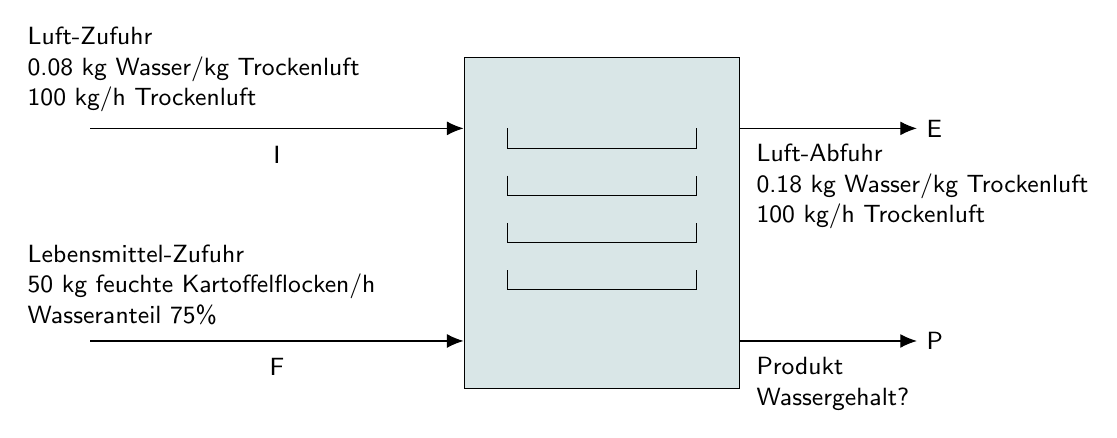
\begin{tikzpicture}[
    >={Latex[length=6pt, width=5pt]}, % Etwas größere Pfeilspitzen (wie zuvor besprochen)
    font={\sffamily \small},
    mainblock/.style={draw, rectangle, minimum width=3.5cm, minimum height=4.2cm, fill=miugray!50}
]

% 1. Hauptblock (Trocknerkammer)
\node[mainblock] (dryer) at (0,0) {};

% 2. Die inneren Fächer (Regale/Bleche) einzeichnen
% Wir nutzen eine Schleife, um die 4 Bleche mit festem Abstand zu zeichnen
\foreach \y in {1.2, 0.6, 0.0, -0.6} {
    \draw ($(dryer.center) + (-1.2,\y)$) -- ++(0,-0.25) -- ++(2.4,0) -- ++(0,0.25);
}

% --- Linke Seite (Eingänge) ---

% Inlet Air (I)
\coordinate (I_start) at (-6.5, 1.2); % Startpunkt weit links
\coordinate (I_end)   at (dryer.west |- I_start); % Endpunkt genau am Rand der Box
\draw[->] (I_start) -- (I_end) node[midway, below=0.1cm] {I};
\node[align=left, anchor=south west, inner sep=0pt, yshift=0.2cm,xshift=-8mm] at (I_start) {Luft-Zufuhr\\0.08 kg Wasser/kg Trockenluft\\100 kg/h Trockenluft};

% Feed (F)
\coordinate (F_start) at (-6.5, -1.5);
\coordinate (F_end)   at (dryer.west |- F_start);
\draw[->] (F_start) -- (F_end) node[midway, below=0.1cm] {F};
\node[align=left, anchor=south west, inner sep=0pt, yshift=0.2cm,xshift=-8mm] at (F_start) {Lebensmittel-Zufuhr\\50 kg feuchte Kartoffelflocken/h\\Wasseranteil 75\% };

% --- Rechte Seite (Ausgänge) ---

% Exit Air (E)
\coordinate (E_start) at (dryer.east |- I_start);
\coordinate (E_end)   at (4, 1.2);
\draw[->] (E_start) -- (E_end) node[right] {E};
% Text rechts unten am Pfeil
\node[align=left, anchor=north west, inner sep=0pt, yshift=-0.2cm,xshift=2mm] at (E_start) {Luft-Abfuhr\\0.18 kg Wasser/kg Trockenluft\\100 kg/h Trockenluft};

% Product (P)
\coordinate (P_start) at (dryer.east |- F_start);
\coordinate (P_end)   at (4, -1.5);
\draw[->] (P_start) -- (P_end) node[right] {P};
% Text rechts unten am Pfeil
\node[align=left, anchor=north west, inner sep=0pt, yshift=-0.2cm,xshift=2mm] at (P_start) {Produkt\\Wassergehalt?};

\end{tikzpicture}
}
\captionsetup{width=.85\linewidth}
\caption{abgeändert, nach Singh \& Heldman, Introduction to Food Engineering}

\end{figure}

\end{minipage}%
\hspace*{4mm}
\begin{minipage}{.55\textwidth}
\antwort{
\footnotesize
\onslide<2->{
Zunächst einmal berechnen wir über die Massenerhaltung die fehlende Größe $P$:}
\begin{align*}
\uncover<3->{I + F &= E + P \\}
\uncover<4->{100 ~\text{kg} \cdot 1,08 + 50 ~\text{kg} &= 100 \cdot 1,18 + P\\}
\uncover<5->{108 ~\text{kg} + 50 ~\text{kg} &=	 118 ~\text{kg} + P \\}
\uncover<5->{P &= 40 ~\text{kg}}
\end{align*}\onslide<6->{
Trockensubstanz in $F$ (die auch in $P$ sein muss):}\onslide<7->{
\begin{align*}
1 - 0,75 &= 0,25 \\
0,25 \cdot 50~\text{kg} &= 12,5~\text{kg}
\end{align*}
}
}


\end{minipage}%



\end{frame}








\begin{frame}
\textbf{Aufgabe 3 b)}\pp
\begin{minipage}{.45\textwidth}
\footnotesize
Kartoffelflocken mit einem Wasseranteil von 75\% werden in einen Gleich\-strom-Durchlauftrockner gegeben. Berechnen Sie
\begin{itemize}
\item den Massenstrom des Produkts
\item den Wassergehalt des Produkts
\end{itemize}


\begin{figure}[h]

\centering
\resizebox{\textwidth}{!}{
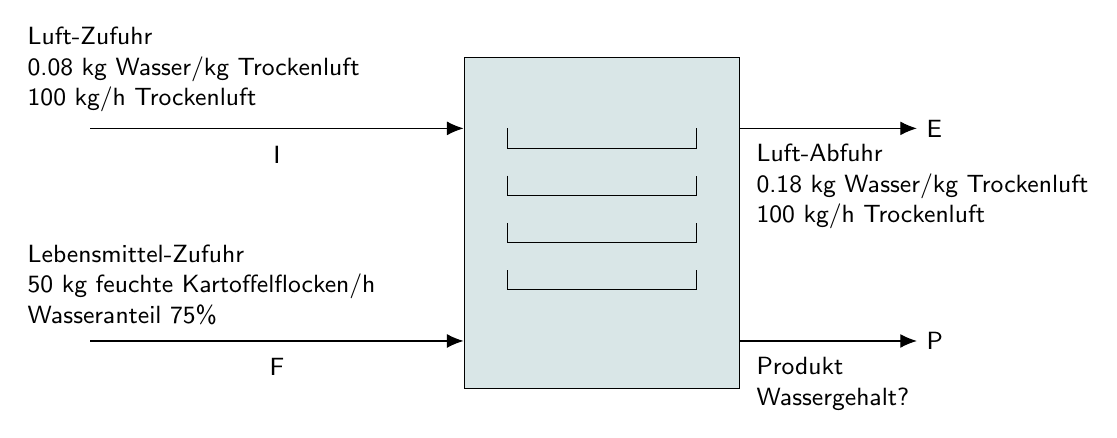
\begin{tikzpicture}[
    >={Latex[length=6pt, width=5pt]}, % Etwas größere Pfeilspitzen (wie zuvor besprochen)
    font={\sffamily \small},
    mainblock/.style={draw, rectangle, minimum width=3.5cm, minimum height=4.2cm, fill=miugray!50}
]

% 1. Hauptblock (Trocknerkammer)
\node[mainblock] (dryer) at (0,0) {};

% 2. Die inneren Fächer (Regale/Bleche) einzeichnen
% Wir nutzen eine Schleife, um die 4 Bleche mit festem Abstand zu zeichnen
\foreach \y in {1.2, 0.6, 0.0, -0.6} {
    \draw ($(dryer.center) + (-1.2,\y)$) -- ++(0,-0.25) -- ++(2.4,0) -- ++(0,0.25);
}

% --- Linke Seite (Eingänge) ---

% Inlet Air (I)
\coordinate (I_start) at (-6.5, 1.2); % Startpunkt weit links
\coordinate (I_end)   at (dryer.west |- I_start); % Endpunkt genau am Rand der Box
\draw[->] (I_start) -- (I_end) node[midway, below=0.1cm] {I};
\node[align=left, anchor=south west, inner sep=0pt, yshift=0.2cm,xshift=-8mm] at (I_start) {Luft-Zufuhr\\0.08 kg Wasser/kg Trockenluft\\100 kg/h Trockenluft};

% Feed (F)
\coordinate (F_start) at (-6.5, -1.5);
\coordinate (F_end)   at (dryer.west |- F_start);
\draw[->] (F_start) -- (F_end) node[midway, below=0.1cm] {F};
\node[align=left, anchor=south west, inner sep=0pt, yshift=0.2cm,xshift=-8mm] at (F_start) {Lebensmittel-Zufuhr\\50 kg feuchte Kartoffelflocken/h\\Wasseranteil 75\% };

% --- Rechte Seite (Ausgänge) ---

% Exit Air (E)
\coordinate (E_start) at (dryer.east |- I_start);
\coordinate (E_end)   at (4, 1.2);
\draw[->] (E_start) -- (E_end) node[right] {E};
% Text rechts unten am Pfeil
\node[align=left, anchor=north west, inner sep=0pt, yshift=-0.2cm,xshift=2mm] at (E_start) {Luft-Abfuhr\\0.18 kg Wasser/kg Trockenluft\\100 kg/h Trockenluft};

% Product (P)
\coordinate (P_start) at (dryer.east |- F_start);
\coordinate (P_end)   at (4, -1.5);
\draw[->] (P_start) -- (P_end) node[right] {P};
% Text rechts unten am Pfeil
\node[align=left, anchor=north west, inner sep=0pt, yshift=-0.2cm,xshift=2mm] at (P_start) {Produkt\\Wassergehalt?};

\end{tikzpicture}
}
\captionsetup{width=.85\linewidth}
\caption{abgeändert, nach Singh \& Heldman, Introduction to Food Engineering}

\end{figure}

\end{minipage}%
\hspace*{4mm}
\begin{minipage}{.55\textwidth}
\antwort{
\footnotesize
\onslide<2->{
Bezogen auf unser getrocknetes Lebensmittel $P$ ist der Anteil an Trockensubstanz $w_{TS}$:}
\onslide<3->{
\begin{align*}
w_{TS} = \frac{12,5~\text{kg}}{40~\text{kg}} = 0,3125
\end{align*}
}
\onslide<4->{
Und somit der Wasseranteil $w_{W}$}
\onslide<5->{
\begin{align*}
w_{W} = 1 - w_{TS} = 1 - 0,3125 &= 0,6875 \\
&= 68,75\%
\end{align*}}
\onslide<6->{
Um eine brauchbare Aussage über den Massenstrom machen zu können, bestimmen wir vorher noch den Wasseranteil pro kg Trockensubstanz:}
\onslide<7->{
\begin{align*}
w_{WTS} = \frac{0,6875}{0,3125} = 2,2
\end{align*}
\RA Der Massenstrom der Kartoffelflocken beträgt 40 kg/h mit einem Wassergehalt von 2,2 kg pro kg Trockensubstanz
}
}


\end{minipage}%



\end{frame}




\begin{frame}

\begin{minipage}{.45\textwidth}
\footnotesize
\textbf{Aufgabe 3 c)}\pp
Mithilfe eines zweistufigen Membranverfahrens wird Saft von 10\% Trockensubstanz (TS) auf 30\% TS aufkonzentriert. Berechnen Sie zunächst die Massenströme von F und W.


\begin{figure}[h]

\centering
\resizebox{\textwidth}{!}{


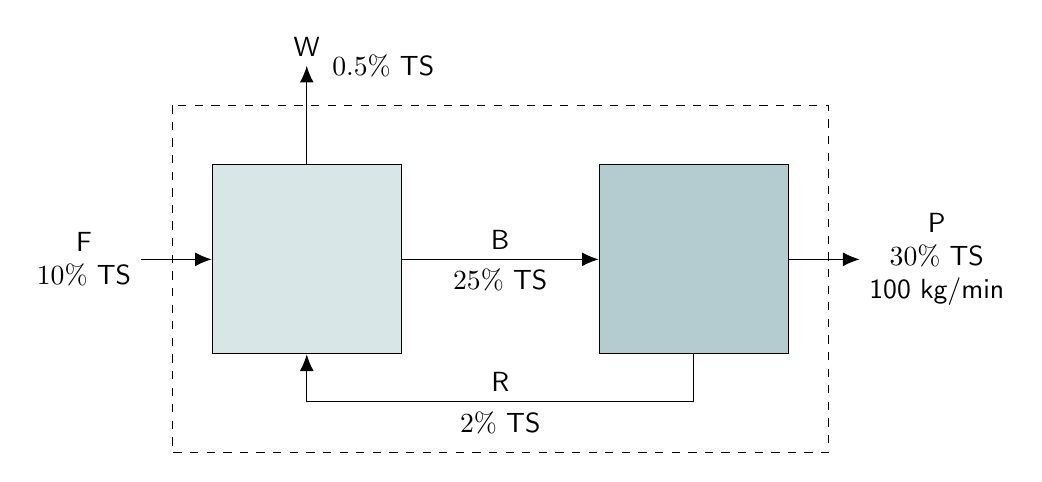
\begin{tikzpicture}[scale=0.5,
    >={Latex[length=6pt, width=5pt]}, % Erzeugt die ausgefüllten dreieckigen Pfeilspitzen
    font=\sffamily, % Nutzt eine serifenlose Schriftart wie im Bild
    block1/.style={draw, rectangle, minimum height=2.4cm, minimum width=2.4cm, fill=miugray!50},
    block2/.style={draw, rectangle, minimum height=2.4cm, minimum width=2.4cm, fill=miugray}
]

% 1. Die beiden Hauptblöcke setzen
\node[block1] (u1) at (0,0) {};
\node[block2, right=2.5cm of u1] (u2) {};

% 2. Systemgrenze (gestrichelte Box)
% Wird zuerst gezeichnet, damit die Box im Hintergrund liegt
\draw[dashed] ($(u1.north west) + (-1cm, 1.5cm)$) rectangle ($(u2.south east) + (1cm, -2.5cm)$);

% 3. Feed-Strom (F)
\draw[<-] (u1.west) -- ++(-1.8cm,0) node[left, align=center] {F\\$10\%$ TS};

% 4. Waste/Wasser-Strom (W) nach oben
\draw[->] (u1.north) -- ++(0, 2.5cm) node[above] {W} node[right, pos=1,xshift=2mm] {$0.5\%$ TS};

% 5. Zwischenstrom (B)
\draw[->] (u1.east) -- (u2.west) node[midway, above] {B} node[midway, below] {$25\%$ TS};

% 6. Produkt-Strom (P)
\draw[->] (u2.east) -- ++(1.8cm,0) node[right, align=center] {P\\$30\%$ TS\\100 kg/min};

% 7. Rückführungs-Strom (Recycle, R)
\draw[->] (u2.south) -- ++(0, -1.2cm) coordinate (r_corner)
          -- (r_corner -| u1.south) node[midway, above] {R} node[midway, below] {$2\%$ TS}
          -- (u1.south);

\end{tikzpicture}
}
\captionsetup{width=.85\linewidth}
\caption{abgeändert, nach Singh \& Heldman, Introduction to Food Engineering}

\end{figure}
\end{minipage}%
\hspace*{6mm}
\begin{minipage}{.55\textwidth}
\antwort{
\footnotesize
\onslide<2->{
Für das ganze System gilt folgende Gleichung:}
\onslide<3->{
\begin{align*}
F = W + P
\end{align*}}
\onslide<4->{
Daher gilt für die Trockensubstanz: }
\onslide<5->{
\begin{align*}
0,1F = 0,005W + 0,3P
\end{align*}}
\onslide<6->{
Da wir wissen, dass $P$ einen Volumenstrom von 100 kg/min hat: }
\onslide<7->{
\begin{align*}
0,1F &= 0,005W + 0,3\cdot100 \\
0,1F &= 0,005W + 30
\end{align*}}
\onslide<8->{
Nun substituieren wir $F$ mit $F = W + P$: }
\begin{align*}
\uncover<10->{0,1(W + P) 	&= 0,005W + 30 \\}
\uncover<11->{0,1(W + 100)&= 0,005W + 30 \\}
\uncover<12->{0,1W + 10	&= 0,005W + 30 \\}
\uncover<13->{0,1W -0,005W&= 30 - 10 \\}
\uncover<14->{0,095W &= 20 \\}
\uncover<15->{W &= 210,5 ~\text{kg/min}\\ \\}
\uncover<16->{F &= 310,5 ~\text{kg/min}}
\end{align*}

}
\end{minipage}%



\end{frame}




\begin{frame}
\textbf{Aufgabe 3 d)}\pp
\begin{minipage}{.45\textwidth}
\footnotesize
Mithilfe eines zweistufigen Membranverfahrens wird Saft von 10\% Trockensubstanz (TS) auf 30\% TS aufkonzentriert. Berechnen Sie nun auch die Massenströme B und R.

\begin{figure}[h]

\centering
\resizebox{\textwidth}{!}{


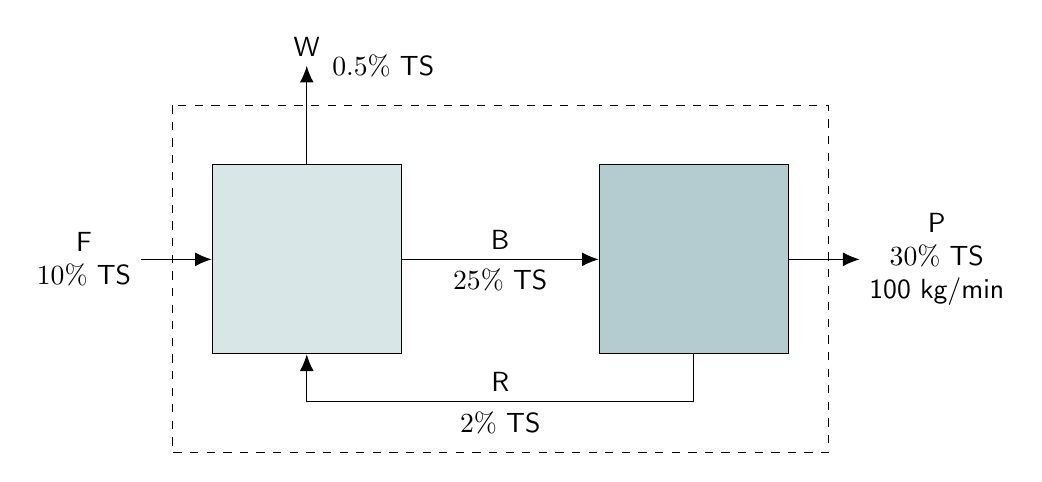
\begin{tikzpicture}[scale=0.5,
    >={Latex[length=6pt, width=5pt]}, % Erzeugt die ausgefüllten dreieckigen Pfeilspitzen
    font=\sffamily, % Nutzt eine serifenlose Schriftart wie im Bild
    block1/.style={draw, rectangle, minimum height=2.4cm, minimum width=2.4cm, fill=miugray!50},
    block2/.style={draw, rectangle, minimum height=2.4cm, minimum width=2.4cm, fill=miugray}
]

% 1. Die beiden Hauptblöcke setzen
\node[block1] (u1) at (0,0) {};
\node[block2, right=2.5cm of u1] (u2) {};

% 2. Systemgrenze (gestrichelte Box)
% Wird zuerst gezeichnet, damit die Box im Hintergrund liegt
\draw[dashed] ($(u1.north west) + (-1cm, 1.5cm)$) rectangle ($(u2.south east) + (1cm, -2.5cm)$);

% 3. Feed-Strom (F)
\draw[<-] (u1.west) -- ++(-1.8cm,0) node[left, align=center] {F\\$10\%$ TS};

% 4. Waste/Wasser-Strom (W) nach oben
\draw[->] (u1.north) -- ++(0, 2.5cm) node[above] {W} node[right, pos=1,xshift=2mm] {$0.5\%$ TS};

% 5. Zwischenstrom (B)
\draw[->] (u1.east) -- (u2.west) node[midway, above] {B} node[midway, below] {$25\%$ TS};

% 6. Produkt-Strom (P)
\draw[->] (u2.east) -- ++(1.8cm,0) node[right, align=center] {P\\$30\%$ TS\\100 kg/min};

% 7. Rückführungs-Strom (Recycle, R)
\draw[->] (u2.south) -- ++(0, -1.2cm) coordinate (r_corner)
          -- (r_corner -| u1.south) node[midway, above] {R} node[midway, below] {$2\%$ TS}
          -- (u1.south);

\end{tikzpicture}
}
\captionsetup{width=.85\linewidth}
\caption{abgeändert, nach Singh \& Heldman, Introduction to Food Engineering}
\label{figure1}

\end{figure}
\end{minipage}%
\hspace*{6mm}
\begin{minipage}{.55\textwidth}
\antwort{
\footnotesize
\onslide<2->{
Ähnlich wie in c) verfahren wir für die Berechnung der Massenströme $B$ und $R$. Es gilt die Beziehung:}
\onslide<3->{
\begin{align*}
F + R = W + B
\end{align*}}
\onslide<4->{Für die Trockensubstanz können wir folgende Faktoren bestimmen:}
\onslide<5->{
\begin{align*}
0,1F + 0,02R = 0,005 W + 0,25 B
\end{align*}}
\onslide<6->{
Nun können wir unsere errechneten Werte für $F$ und $W$ einsetzen und nach R auflösen:}

\begin{align*}
\uncover<7->{0,1\cdot 310,5 + 0,02 R &= 0,005 \cdot 210,5 + 0,25 B \\}
\uncover<8->{31,05 + 0,02 R 			&= 1.0525 + 0,25 (R + P) \\}
\uncover<9->{31,05 + 0,02 R			&= 1.0525 + 0,25 R + 25 \\}
\uncover<10->{4,9975					&= 0,23 R \\}
\uncover<11->{R 						&= 21,73~\text{kg/min}\\ \\}
\uncover<12->{B 						&= R + P = 121,73 ~\text{kg/min}}
\end{align*}
}
\end{minipage}%



\end{frame}





\begin{frame}

\begin{center}
\LARGE
Vielen Dank fürs Zuhören \par 
\normalsize
und bis nächste Woche.. :) \pp
%\includegraphics[width=5cm]{F://LaTeX-Files/pngs/danja}
\end{center}
\end{frame}

\end{document}
